\documentclass[technicalreport]{ieicej}
%\documentclass[technicalreport,usejistfm]{ieicej}
\usepackage[dvipdfmx]{graphicx}
\usepackage{latexsym}
%\usepackage[fleqn]{amsmath}
\usepackage{amsmath}
\usepackage{amssymb}
\usepackage{multirow,eepic}
\usepackage{cite}
\usepackage{mediabb}
\usepackage{url}
\usepackage{comment}
\usepackage{epsfig}
\usepackage{subfig}
\setlength{\oddsidemargin}{-9mm}
\setlength{\evensidemargin}{-9mm}
\setlength{\topmargin}{-4mm}
%\renewcommand{\topfraction}{1.0}
%\renewcommand{\bottomfraction}{1.0}
%\renewcommand{\dbltopfraction}{1.0}
%\renewcommand{\textfraction}{0.01}
%\renewcommand{\floatpagefraction}{1.0}
%\renewcommand{\dblfloatpagefraction}{1.0}
\setcounter{topnumber}{5}
\setcounter{bottomnumber}{5}
\setcounter{totalnumber}{10}

\newcommand{\sij}{(i,j)}
\newcommand{\sijk}{(i,j,k)}
\newcommand{\mN}{{\mathcal N}}
\newcommand{\pijk}{p^{(i,j,k)}}
\newcommand{\rd}{r^{\sij}_{\rm d}}
\newcommand{\ru}{r^{\sij}_{\rm u}}
\newcommand{\rijk}{r^{(i,j,k)}}
\newcommand{\etau}{\eta_{\rm u}^{(j)}}
\newcommand{\mthc}{\mathcal C}
\newcommand{\mthni}{{\mathcal N}_i}
\newcommand{\mthnj}{{\mathcal N}_j}
\newcommand{\mthnk}{{\mathcal N}_k}
\def\coloneqq{\mathrel{\mathop:}=}

\jtitle{上りOFDMAによる全二重通信無線LANの遅延時間削減}
%\jsubtitle{}
\etitle{Station Selection Scheme for In-Band Full-Duplex WLAN with UL-OFDMA for Reducting Transmission Delay}
%\esubtitle{}
 \alignorder=4
 \breakauthorline{4}

\authorlist{%
 \authorentry[info16@imc.cce.i.kyoto-u.ac.jp]{飯田 直人}{Naoto Iida}{^1}
 \authorentry{西尾 理志}{Takayuki NISHIO}{^1}
 \authorentry{守倉 正博}{Masahiro MORIKURA}{^1}
 \authorentry{山本 高至}{Koji YAMAMOTO}{^1}
 \authorentry{鍋谷 寿久}{Toshihisa Nabetani}{^2}
 \authorentry{青木 亜秀}{Tsuguhide Aoki}{^2}
 }

\affiliate[^1]{京都大学大学院情報学研究科\hskip1zw
  〒606-8501 京都市左京区吉田本町}
 {Graduate School of Informatics, Kyoto University\hskip1em
  Yoshida-honmachi, Sakyo-ku, Kyoto,
  606-8501 Japan}
\affiliate[^2]{株式会社東芝 研究開発センター\hskip 1zw 〒212-8582 神奈川県川崎市幸区小向東芝町1}
  {Corporate Research \& Development Center, TOSHIBA Corporation\hskip1em
   1 Komukaitoshiba-cho, Saiwai-ku, Kawasaki-shi, Kanagawa 212-8582, Japan}

\begin{document}
\begin{jabstract}
	無線LANの大容量化に向けて,自己干渉除去技術により送信と受信を同一帯域で同時に行う全二重通信無線LANが有望である.
	特に,1台のAP(Access Point)とAPへの上り通信を行うSTA(Station),
	APからの下り通信を受信するSTAの3台によるUFD(user-multiplexing Unidirectional Full-Duplex)通信は自己干渉除去技術を持たないSTAにも適用可能であるという利点がある.
	しかし,UFD通信では下り通信の送信機会が大きく増加しシステムスループットは向上するものの,
	ユーザ間干渉による伝送速度の低下やSTAの送信頻度の低下のため,STAからの上り通信の遅延時間が大きく増加する問題がある.
	STAの上り送信の遅延時間削減に向け,上りOFDMAを用いた全二重通信無線LANにおける送受信STA選択手法を提案する.
	上りOFDMAにより,1回の送信機会に複数のSTAの同時送信を可能とし,STAの送信機会を向上させ遅延時間を削減する.
	送受信をおこなうSTA組の決定問題を最適化問題として定式化し,APは本最適化問題より各STAの選択確率を決定する.
	シミュレーション評価により,提案方式はシステムスループットを大きく低下させることなく遅延時間を半二重通信と同等まで削減できることを示した.
\end{jabstract}
\begin{jkeyword}
	全二重通信無線LAN,ユーザ間干渉,遅延時間, OFDMA
\end{jkeyword}
\begin{eabstract}
	Self-interference cancellation techniques enable in-band full-duplex wireless local area networks (WLANs), where nodes can  transmit and receive simultaneously in the same frequency band.
	In particular, user-multiplexing unidirectional full-duplex (UFD) communication, where a full-duplex access point (AP) transmits a frame to a station (STA) and receives a frame from another STA, is a promising technology for broadband WLANs, since UFD is applicable for the conventional STAs without self-interference cancellation capability.
	However, the UFD communication increases an uplink transmission delay.
	In this paper, we propose a station selection scheme where combination of sender and receiver STAs are adaptively selected in order to increase a throughput and reduce the transmission delay.
	The scheme uses the UFD communication and uplink OFDMA system, and increases transmission opportunities of STAs.
	Simulation results show that the proposed scheme reduces the delay to the same level as the half-duplex system.

\end{eabstract}
\begin{ekeyword}
	full-duplex wireless LAN, inter-user interference, delay, OFDMA
\end{ekeyword}

\titlepagebaselinestretch{0.95}

\maketitle

\renewcommand{\baselinestretch}{0.99}\selectfont

\section{はじめに}
	近年,無線LAN(Local Area Network)が急速に普及し,急増するトラヒックにより2.4\,GHz帯は逼迫しており,
	近い将来5\,GHz帯の逼迫も懸念されることから,無線LANのさらなる大容量化は急務である.
	大容量化を実現する方法の一つとして,送信と受信を同じ周波数帯で同時に行う全二重通信無線LANが有望である.
	全二重通信無線LANでは上り通信と下り通信を同一帯域で同時に行うため,システムスループットを向上させることができる.
	全二重通信無線LANには,図\ref{fig:topology}\subref{fig:bfd}に示すAP(Access Point)からの下り通信を受信するSTA(station)と上り通信を行うSTAが同一である双方向全二重(BFD: Bidirectional Full-Duplex)通信と,
	図\ref{fig:topology}\subref{fig:ufd}に示すような上り通信を行うSTAと下り通信を受信するSTAが異なる全二重(UFD: user-multiplexing Unidirectional Full-Duplex)通信がある.
%	本稿では,このUFD通信のうち,STA $j$からSTA $i$へのAPを介してのリレー通信ではなく,
%	STA $i$,$j$はそれぞれコアネットワークからの下りトラヒックの受信,コアネットワークへの上りトラヒックの送信を行っているものを扱う.
%	UFD通信にはSTAにおける自己干渉が存在しないため,
%	BFD通信と異なり自己干渉除去技術を持たない従来のSTAにも適用可能であるという利点がある.
%	このUFD通信を用いた無線LANでは二つの干渉が問題となる.
%	一つは,送受信を行っているAPにおいて,送信信号が所望の受信信号に干渉を及ぼす自己干渉である.
%	自己干渉を受けるAPにとって干渉波は自身の送信信号であり既知であるため,
%	自己干渉除去技術を用いて自己干渉を最大110\,dB除去できることが示されている~\cite{fdmac, stanford1}.
	全二重通信では送信と受信を同時に行うため,送信信号が所望受信信号に干渉を及ぼす自己干渉が生じる.
	自己干渉波は既知の信号であることを用いて干渉を除去する技術が検討されており,最大で110\,dB除去できることが示されている~\cite{fdmac, stanford1}.
	BFD通信では自己干渉がAPとSTAの両方で生じる.
	そのため,干渉除去機能を有しない既存の無線LAN機器には適用できない.
	UFD通信ではSTAにおける自己干渉が生じないため, 自己干渉除去機能を持たない従来のSTAにも適用可能であるという利点がある.
	一方で,UFD通信ではSTA $j$の送信信号が他方のSTA $i$の受信信号に干渉を及ぼすユーザ間干渉が生じる.
	ユーザ間干渉は,干渉を受けるSTA $i$にとって干渉波がSTA $j$の送信する未知の信号であるため,
	自己干渉のように除去することが困難である.
	\par
	このユーザ間干渉の影響を低減するためには,干渉の大きさを考慮して上り通信を行うSTAと下り通信を受信するSTAの適切な組み合わせを選択することが必要である~\cite{promac}.
	これまで著者らはUFD通信における送受信STA選択手法を最適化問題として定式化し,システムスループットとSTA間の送信機会に関する公平性を両立するアクセス制御方式を提案している~\cite{promac_fair}.
	\par
	しかし,APと比べSTAのデータフレーム長が短い場合に,UFD通信では半二重通信と比較して,
	上り通信を行うSTAの遅延時間が増大するという課題が残っている.
	これは,図\ref{fig:problem}に示すように,UFD通信ではユーザ間干渉により伝送速度が低下するため一回の送信時間が増加し,
	かつ,下り通信の送信頻度が増加するため,半二重通信と比較してSTAの送信頻度が低下するためである.
	上り通信の遅延時間の増大は,TCP(Transmissioin Control Protocol)下り通信におけるTCP-ACK(Acknowledgement)パケットの遅延を増加させ,
	結果的にTCPスループットの低下が生じる~\cite{rtt}.
	\begin{figure}[t]
		\centering
		\subfloat[BFD通信]{
			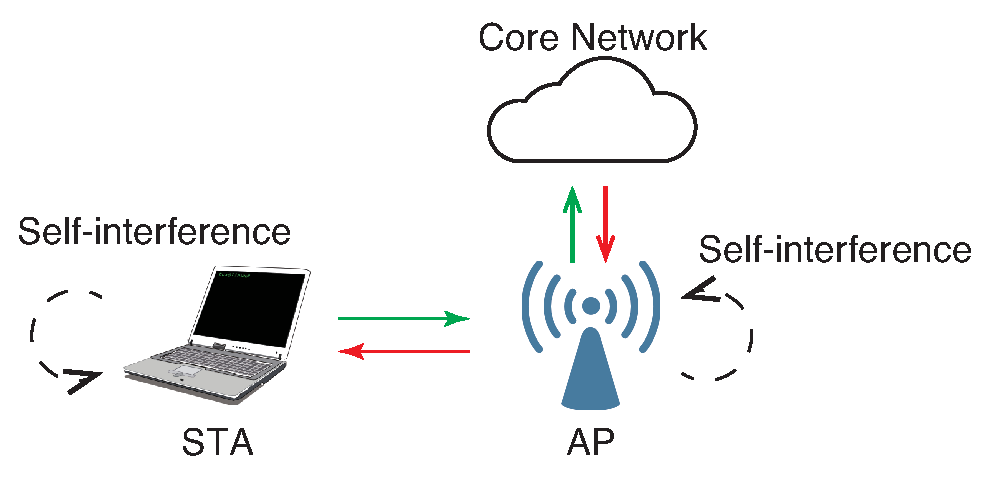
\epsfig{file=fig/bfd.eps, scale=0.35}
			\label{fig:bfd}
		}
		\\
		\subfloat[UFD通信]{
			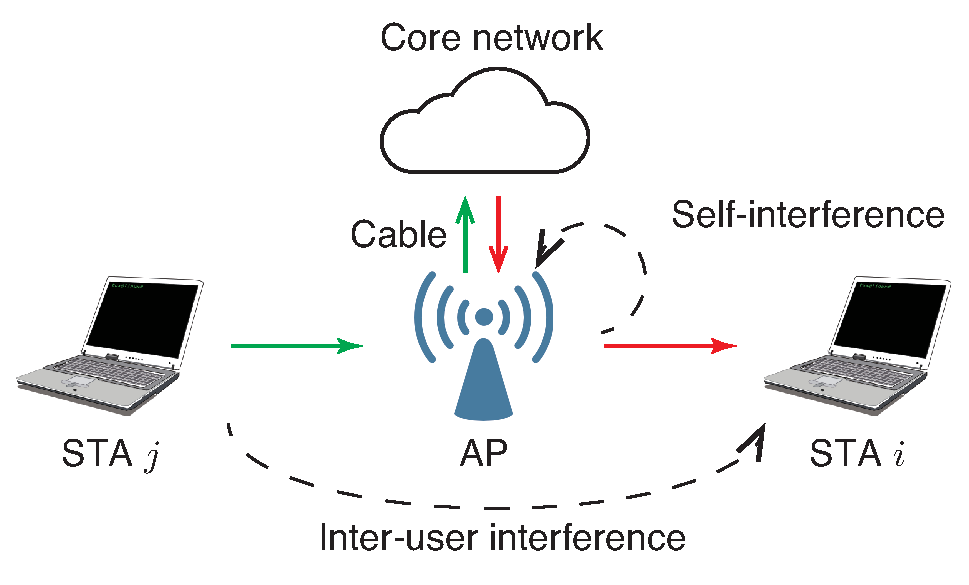
\epsfig{file=fig/ufd.eps, scale=0.35}
			\label{fig:ufd}
		}
		\caption{全二重通信の適用例}
		\label{fig:topology}
	\end{figure}
	\begin{figure}[t]
		\centering
		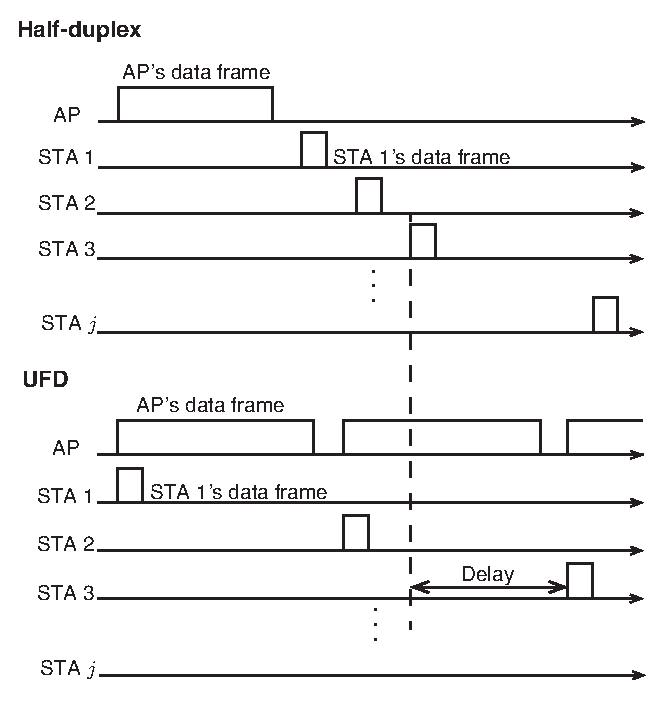
\epsfig{file=fig/problem.eps, scale=0.65}
		\caption{半二重通信とUFD通信におけるSTAの送信機会}
		\label{fig:problem}
	\end{figure}
	\par
	本稿では,遅延時間削減に向け,UFD通信の上り通信へOFDMAを適用した無線LANと本無線LANにおける送受信STA選択手法を提案する.
	図\ref{fig:ofdma}にシステムモデルを示す.
	OFDMAとは周波数チャネルを複数に分割し,サブキャリアを複数のユーザに割り当て,時間的に並列伝送する方式である.
	現在策定が進められているIEEE 802.11axにおいて,OFDMAは,短いフレームの並列伝送による周波数利用効率の向上や,
	TCP-ACKの遅延時間削減によるTCPスループットの向上を実現する技術として期待されている~\cite{ofdma}.
	提案方式では,OFDMA導入により,送受信STAの選択において複数の上り通信STAを選択可能とし,
	STAの送信機会を向上することで遅延を削減する.
	本稿では,~\cite{promac_fair}で提案する送受信STA選択最適化問題を拡張し,上りOFDMAに対応したSTA選択を可能とする.
	提案手法では,半二重通信,UFD通信,上りOFMDA,UFD通信と上りOFDMAの組み合わせの4つの通信方式を適応的に切り替え,STA選択を行う.
	送受信STA組を適応的に選択することで,干渉が大きくUFD通信を行えないような位置にあるSTAは半二重通信を行い,
	干渉が小さく,大きなスループットを期待できるSTAにはUFD通信を用い,
	多くのSTAへ送信機会を与えたい場合はOFDMAを用いるといったような状況に応じた制御が可能となる.
	\begin{figure}[t]
		\centering
		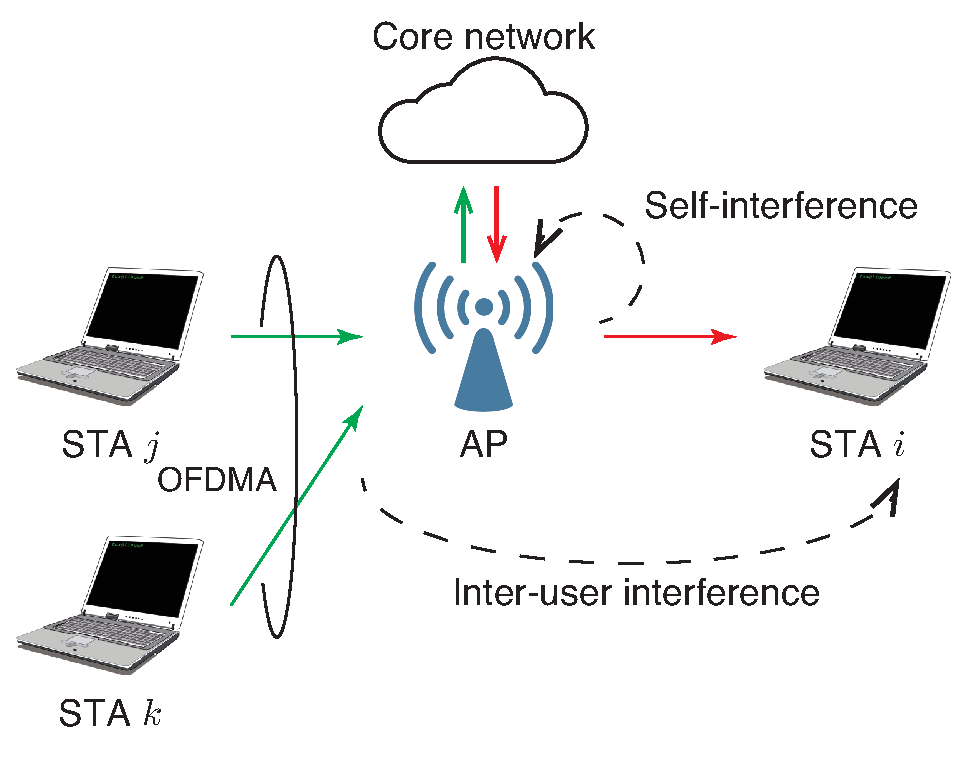
\epsfig{file=fig/ofdma.eps, scale=0.35}
		\caption{UFD通信とOFDMAの組み合わせ}
		\label{fig:ofdma}
	\end{figure}
	\par
	本稿の構成は以下のとおりである.第2章で本稿で扱うシステムモデルについて述べ,
	第3章において提案方式について述べる.
	第4章では提案方式の有効性をシミュレーションによって評価し,最後に第5章でまとめとする.

\section{システムモデル}\label{seq:system}
	\begin{figure}[t]
		\centering
		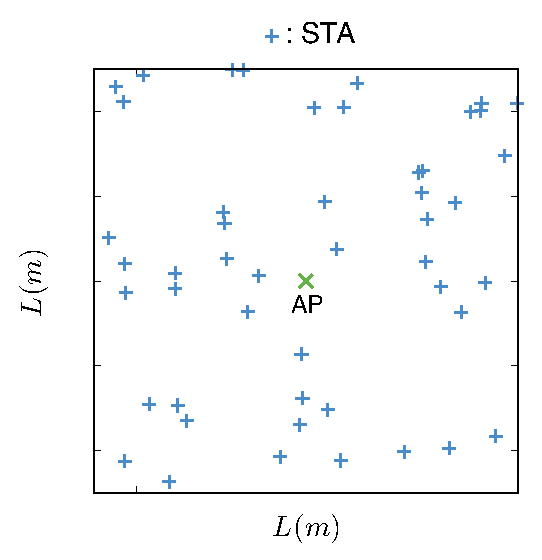
\epsfig{file=fig/pos.eps, scale=0.4}
		\caption{APとSTAの配置の一例}
		\label{fig:model}
	\end{figure}

	図\ref{fig:model}にAPとSTAの配置の一例を示す.
	1台のAPが$L$\,m四方の領域の中心に設置され,その周りに$N$台のSTAがランダムに配置されているとする.
	それらSTAのインデックス集合を$\mN=\{1,2,...,N\}$とする.
	OFDMAによる多重化は簡単のため二多重までとし,半二重通信,UFD通信で用いるチャネルを2台のSTAが二等分して用いる.
	この$N$台のSTAの中から,図\ref{fig:ofdma}のようにAPからの下り通信を受信するSTA $i$と,
	APへの上り通信を行うSTA $j$,$k$を選び出す.
	このとき,STAの組み合わせを$\sijk$と表現し,$i,\ j,\ k \in \{0\}\cup \mN$とする.
	STAは自己干渉除去技術を持たずBFD通信はできないとし,$i\neq0$のときには$i\neq j$かつ$i\neq k$とする.
	また,$i$,$j$,$k$の全てが0になることはないものとする.
	$i$,$j$,$k$のそれぞれが取る値によって以下の通信方式を定義し,切り替え可能であるものとする.
	\begin{itemize}%\setlength{\leftskip}{10pt}
		\item ($i=0\land jk=0\land j+k\neq0)\lor (i=0\land j=k\neq0)$\par
			\hspace*{15pt}上りの半二重通信
		\item $i\neq0\land j=k=0$\par
			\hspace*{15pt}下りの半二重通信
		\item $(i\neq0\land jk=0 \land j+k\neq0)\lor(i\neq0\land j=k\neq0)$\par
			\hspace*{15pt}UFD通信
		\item $i=0\land jk\neq0 \land j\neq k$\par
			\hspace*{15pt}上りOFDMA
		\item $i\neq0 \land jk\neq0 \land j\neq k$\par
			\hspace*{15pt}OFDMAとUFD通信の組み合わせ
	\end{itemize}
	\par
	また,STAの組み合わせを決定する際に用いる推定スループットには,上り下り通信のそれぞれのSINR(Signal-to-Interference plus Noise power Ratio)に対するシャノン容量を用いる.ただし,$B$は通信に用いる帯域幅である.
	\begin{equation}
		{\rm Shannon\ capacity}=B\log_2(1+{\rm SINR}) \label{eq:capacity}
	\end{equation}
	\par
	本稿では,図\ref{fig:standby}に示すようにSTAの遅延時間を,あるデータフレームに対しそのフレームがSTAの送信バッファの先頭に到着した時刻から送信機会を獲得しそのフレームの送信が開始した時刻までの経過時間とする.
	これは,輻輳制御やバッファ制御の影響を排除した無線メディアアクセス制御における遅延を評価するためである.
	\begin{figure}[t]
		\centering
		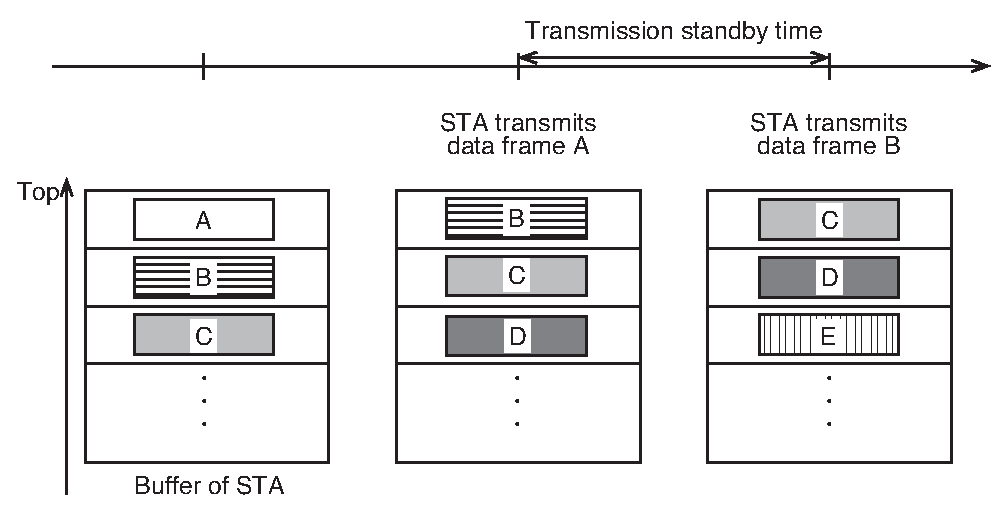
\epsfig{file=fig/standby.eps, scale=0.45}
		\caption{遅延時間の定義}
		\label{fig:standby}
	\end{figure}



%\section{従来方式の問題点とその原因}\label{sec:problem}
%	従来のUFD通信を用いる方式では,半二重通信である場合に比べて遅延時間が増大してしまう.
%	本節では遅延時間の増加という問題点とその原因について述べる.
%	\subsection{遅延時間の増加}
%		\begin{figure}[t]
%			\centering
%			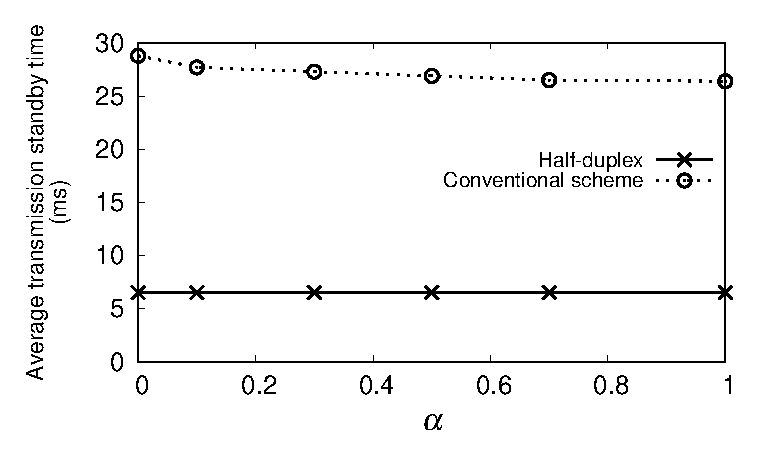
\epsfig{file=graph/delay_sub.eps, scale=0.6}
%			\caption{半二重通信と従来方式における送信待機時間}
%			\label{fig:delay_sub}
%		\end{figure}
%		図\ref{fig:delay_sub}に半二重通信のみを用いる場合と半二重通信とUFD通信を併用する従来方式~\cite{promac_fair}の場合の
%		STAの平均送信待機時間を示す.
%		ただし,送信待機時間とは各STAにおいてあるデータフレームがバッファの先頭に到着してからの経過時間であり,
%		$\alpha$は目的関数における送信待機時間の.影響を調整するパラメータである.
%		送信待機時間が半二重通信の場合と比べて,従来方式は4倍以上の値となっていることがわかる.
%	\subsection{伝送速度の低下}
%		本節では送信待機時間が半二重通信の場合と比べて大きくなってしまう原因について述べる.
%		APの送信電力を$P_{\rm AP}$,STA $j$の送信電力を$P_j$とし,
%		AP-STA $i$間,AP-STA $j$間,STA $i$-$j$間のチャネル係数をそれぞれ$h_{{\rm AP},i}$,$h_{{\rm AP},j}$,$h_{i,j}$とし,
%		雑音電力を$\sigma^2$とすると,半二重通信の場合における上下通信のSNRはそれぞれ,
%		\begin{align}
%			{\rm SNR_{\rm d}^{\rm h}} &= \cfrac{P_{\rm AP}|h_{{\rm AP},i}|^2}{\sigma^2} \label{eq:hd}\\
%			{\rm SNR_{\rm u}^{\rm h}} &= \cfrac{P_j |h_{{\rm AP},j}|^2}{\sigma^2}\label{eq:hu}
%		\end{align}
%		となる.
%		一方,UFD通信の場合の上下通信のSINRはそれぞれ,
%		\begin{align}
%			{\rm SINR_{\rm d}^{\rm f}} &= \cfrac{P_{\rm AP} |h_{{\rm AP},i}|^2}{\sigma^2+P_j'|h_{i,j}|^2}\label{eq:fd}\\
%		\end{align}
%		となる.
%		ただし,$P_j'$は~\cite{promac}による送信電力制御を行った場合のSTA $j$の送信電力であり$P_j'\leq P_j$である.
%		また,$h_{\rm AP,AP}$はAPの送信信号がAP自身によって受信されるまでの伝搬路のチャネル係数に,
%		自己干渉除去技術による干渉除去の効果を加味した値である.
%		\par
%		式\eqref{eq:hd}と\eqref{eq:fd}の比較,式\eqref{eq:hu}と\eqref{eq:fu}の比較からわかるように,
%		UFD通信における上下通信のSINRは,半二重通信の場合のSNRと比べて干渉と送信電力制御による送信電力低下の分だけ悪化する.
%		これにより,UFD通信では,半二重通信の場合に比べて上下通信それぞれの伝送速度が低下してしまう.

\section{提案方式}\label{sec:propose}
	本節では,遅延時間の増大を防ぐため,上り通信をOFDMAを用いて多重化することを提案する.
	OFDMAを用いてSTAの送信機会を増加させることで遅延時間を削減する.
	STA決定手法は従来方式~\cite{promac_fair}における手法をOFDMAを適用できるように拡張する.
	また,本章で述べる部分以外のMAC(Media Access Control)プロトコルは~\cite{promac}に従う.

	\subsection{送受信STA組決定手法の概要}\label{sec:opt}
		\begin{figure}[t]
			\centering
			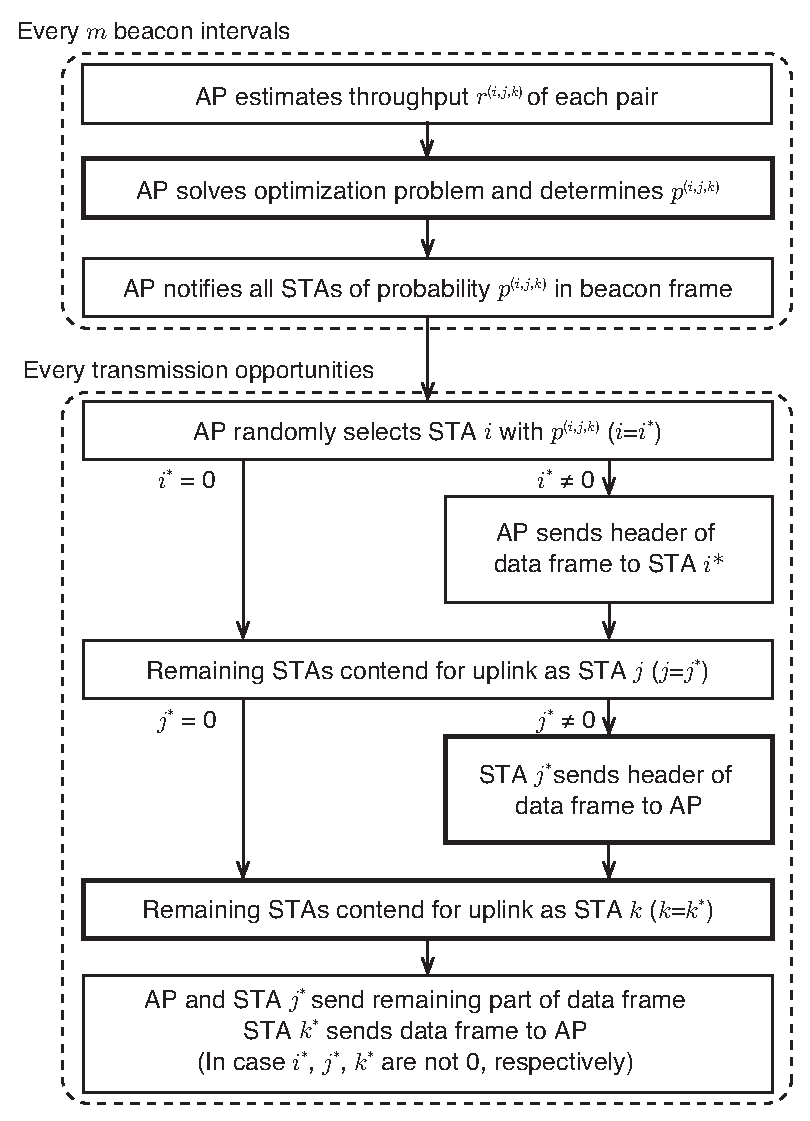
\epsfig{file=fig/proccess.eps, scale=0.5}
			\caption{送受信STA選択手法の手順}
			\label{fig:process}
		\end{figure}
		%まず,STAの組み合わせの集合${\mathcal C}_{\rm half}$,${\mathcal C}_{\rm UFD}$,${\mathcal C}_{\rm OFDMA}$,${\mathcal C}_{\rm OFDMA-UFD}$,${\mathcal C}$を以下のように定義する.
		%\begin{align}
		%	&{\mathcal C}_{\rm half} \coloneqq \{\sijk : i=0\cap ((jk=0 \cap j+k\neq0) \cup(j=k\neq0)),\ \rijk >\epsilon\} \\
		%	&{\mathcal C}_{\rm UFD} \coloneqq \{\sijk : i,j\in{\mathcal N},\ i\neq j,\ r^{\sij}_{\rm d},\ r^{\sij}_{\rm u}>\epsilon\} \\
		%	&{\mathcal C}_{\rm OFDMA} \coloneqq \{\sijk : i=0,\ jk\neq0\in{\mathcal N},\ r^{\sij}_{\rm d},\ r^{\sij}_{\rm u}>\epsilon\}
		%\end{align}
		本手法の手順は図\ref{fig:process}の通りである.
		太枠で示した部分が,OFDMAの適用にあたって拡張を行った部分である.
		本手法は各STA組毎の干渉の大きさや各STAの遅延時間をもとに,通信方式の選択と送受信を行うSTA組を適応的に決定することが目的である.
		そのため,まずAPは全STA組に対してその組み合わせで通信が行われた場合のスループットを推定する.
		また,各STAの送信待機時間を事前に収集しておく.
		ただし,送信待機時間とは各STAにおいてあるデータフレームがバッファの先頭に到着してから現在時刻までの経過時間である.
		APは推定されたスループットと各STAの送信待機時間を用いて最適化問題を解き,各STA組で通信が行われる確率を求める.
		最適化問題の目的関数は,システムスループットを大きくし,かつ,STAの遅延時間を削減するため,
		前述の推定スループットが大きいSTA組や送信待機時間が長いSTAを含むSTA組が選ばれやすくなるよう設計する.
		推定スループットは干渉の大きさや用いる伝送速度によって変化し,送信待機時間はSTAが送信を行う度に変化する上,
		STAの増減も起こる.
		そういった状況の変化に対応するために,APは定期的にスループットの再推定と送信待機時間の再収集を行い,
		最適化問題を解き直すことで確率を更新する.
		得られた確率はビーコンフレームによって全てのSTAへ通知される.
		\par
		次に,得られた確率を用いてSTA組を決定する.
		APは下り通信の送信先となるSTA $i$を確率的に決定する.
		選ばれたSTAをSTA $i^*$とし,APは送信先がSTA $i^*$であることを通知するため,データフレームのヘッダ部分を送信する.
		続いて,全てのSTAはAPから通知された確率をもとにコンテンションウィンドウを設定し,
		CSMA/CA (Carrier Sence Multiple Access with Collision Avoidance)のバックオフアルゴリズムを用いた競合を行い,
		STA $j$,$k$が順に決定される.
		決定したSTAをそれぞれSTA $j^*$,$k^*$とし,
		STA $j^*$は自身が送信権を獲得したことを通知するため,データフレームのヘッダ部分を送信する.
		最後に,APとSTA $j^*$はデータフレームの残りの部分を,STA $k^*$はデータフレームを送信する.

	\subsection{送受信STA組決定手法の詳細}
		本節では前節で述べた各手順について詳細を述べる.
		従来方式~\cite{promac_fair}に対しては,OFDMAを適用しSTA $k$を追加するために,最適化問題の拡張とSTA $k$の決定手順追加がなされている.
		\par
		まず,APは全ての組み合わせ$(i,j,k)$に対してスループット$r^{(i,j,k)}_{\rm d}$,$r^{(i,j,k)}_{\rm u1}$,$r^{(i,j,k)}_{\rm u2}$を推定する.
		ただし,$r^{(i,j,k)}_{\rm d}$はAPからSTA $i$への下り通信の推定スループット,$r^{(i,j,k)}_{\rm u1}$,$r^{(i,j,k)}_{\rm u2}$はSTA $j$,$k$による上り通信の推定スループットである.
		ここで,全組み合わせの集合から最低伝送速度の所要SINRを満たさない通信が含まれている組み合わせを除外した集合を$\mthc$とし,
		$\mthc$の要素$\sijk$に含まれる$i$,$j$,$k$の集合をそれぞれ$\mthni$,$\mthnj$,$\mthnk\subseteq \{0\}\cup{\mathcal N}$とする.
		APは$\rijk=r^{(i,j,k)}_{\rm d}+r^{(i,j,k)}_{\rm u1}+r^{(i,j,k)}_{\rm u2}$と,
		上り通信を行うSTA $j$,$k$の送信待機時間$d^{(j)}$,$d^{(k)}$を用いて以下の最適化問題を解き,
		各組み合わせで通信が行われる確率$p^{(i,j,k)}$を求める.

		\begin{align}
			&{\mathcal P}_1: && {\rm max} \sum_{(i,j,k)\in{\mathcal C}} p^{(i,j,k)}r^{(i,j,k)}(d^{(j)}+d^{(k)})^{\alpha} &&&&&&\\
			&{\rm subject\ to} && \sum_{k\in\mthnk} \sum_{j\in\mthnj} p^{(i,j,k)} \geq \eta_{\rm d}^{(i)},\ \forall i\in {\mathcal N} \label{eq:etad} \\
			&&& \sum_{j\in\mthnj} \sum_{i\mthni} p^{(i,j,l)}+\sum_{k\in\mthnk} \sum_{i\in\mthni} p^{(i,l,k)} \nonumber\\
			&&&\qquad\qquad- \sum_{i\in\mthni} p^{(i,l,l)} \geq \eta_{\rm u}^{(l)},\ \forall l\in {\mathcal N} \label{eq:etau} \\
			&&& \sum_{(i,j,k)\in{\mathcal C}} p^{(i,j,k)}=1 \\
			&{\rm variables:} &&p^{(i,j,k)} \in {\mathbb R}_{\geq 0},\forall(i,j,k)\in {\mathcal C}
		\end{align}
		\par
		目的関数は推定スループットが大きく,送信待機時間が大きなSTAを含む組ほど通信を行う確率が高くなるようにするため,
		確率$\pijk$,推定スループット$\rijk$とSTA $j$,$k$の送信待機時間の和$d^{(j)}+d^{(k)}$の積として設計されている.
		また,システムスループットとSTAの遅延時間の優先度を調整するため,
		パラメータ$\alpha$を目的関数に導入し,$d^{(j)}$,$d^{(k)}$の影響の大小を調節できるようにする.
		$\alpha$が大きいほど遅延時間を優先し,送信機会を得られていないSTAを含む組が選ばれやすくなる.
		さらに,選ばれる確率が0となるSTA組みが発生しないよう式\eqref{eq:etad},\eqref{eq:etau}によって下限を設定する.
		第一の制約条件式\eqref{eq:etad}はあるSTA $i$が下り通信の送信先となる確率を$\eta_{\rm d}^{(i)}$以上とする条件であり,
		第二の制約条件式\eqref{eq:etad}はあるSTA $l$がSTA $j$または$k$として上り通信を行う確率を$\eta_{\rm u}^{(l)}$以上とする条件である.
		$\eta_{\rm d}^{(i)}$,$\eta_{\rm u}^{(l)}$は0より大きく,それぞれのトラヒックに比例した値が設定される.
		APによって算出された確率$\pijk$はビーコンフレームによって全てのSTAに通知される.
%		この最適化問題で用いられる$d^{(j)}$,$d^{(k)}$は時間変化する値であるため,
%		APは数回のビーコンフレーム送信毎に最新の$\rijk$,$d^{(j)}$,$d^{(k)}$をもとに最適化問題を解き,
%		確率$\pijk$の更新を行う.
		\par
		次に,STA $i$,$j$,$k$を決定する.
		まず最初に,APが下り通信の受信STAとなるSTA $i$の決定を行う.
		APは以下の式に従って,各STAが下り通信の送信先となる確率$p_{\rm d}^{(i)}$を求める.
		\begin{equation}
			p_{\rm d}^{(i)}= \sum_{k\in\mthnk}\sum_{j\in\mthnj}p^{(i,j,k)}, \ \forall i \in \{0\}\cup{\mathcal N}
		\end{equation}
		APはこの確率$p_{\rm d}^{(i)}$に従って確率的にSTA $i$を選択する.
		確率的に決定されたSTAをここではSTA $i^*$とする.
		このとき$i^*=0$であれば,下り通信が行われないことを示す.
		全てのSTAは以降の手順においてAPの送信先を知っておく必要があるため,STA $i^*$の決定後,
		APはSTA $i^*$へ送信するデータフレームのヘッダ部分のみを送信し,送信先がSTA $i^*$であることを全STAに通知する.
		\par
		続いて,CSMA/CAのバックオフアルゴリズムを用いた競合によってSTA $j$を決定する.
		まず,バックオフカウンタを設定するために,STA $i^*$以外のSTAは以下の確率を計算する.
		\begin{align}
			p_{\rm u1}^{(i^*,j,k)}=\left(\sum_{k\in\mthnk} p^{(i^*,j,k)}\right) / p_{\rm d}^{(i)},\ \forall j \in \{0\}\cup{\mathcal N}\backslash \{i^*\}
		\end{align}
		これは,APがSTA $i^*$へ送信することが決まった上で,各STAが上り通信を行う条件付き確率である.
		この確率をもとに,各STAはコンテンションウィンドウサイズ${\rm CW}^{(i^*,j,k)}_{\rm u1}$を
		\begin{equation}
			{\rm CW}^{(i^*,j,k)}_{\rm u1} = \lceil 1/p_{\rm u1}^{(i^*,j,k)} \rceil
		\end{equation}
		と設定する.
		ただし,$\lceil x \rceil$は$x$を超えない最大の整数である.
		各STAは$[0,\ {\rm CW}^{(i^*,j,k)}_{\rm u1}]$の一様分布から生成されるバックオフカウンタ$w_{\rm u1}^{(i^*,j,k)}$を設定し,
		CSMA/CAのバックオフアルゴリズムを用いてバックオフカウンタを1ずつ減らす.
		その結果,最初にカウンタが0となったSTAが上り通信を行う.
		ここで,上り通信の送信権を獲得したSTAをSTA $j^*$とし,
		$j^*=0$のときはSTA $j$による上り通信は行われないことを示す.
		STA $j^*$は自身が送信権を獲得したことを他のSTAに知らせるため,
		APへ送信するデータフレームのヘッダ部分のみを送信する.
		\par
		最後にSTA $k$の決定を行う.
		STA $i^*$以外のSTAは,STA $j$の決定の際と同様に以下の条件付き確率を求める.
		\begin{align}
			p_{\rm u2}^{(i^*,j^*,k)}=p^{(i^*,j^*,k)} / \left(\sum_{k\in\mthnk} p^{(i^*,j^*,k)}\right), \nonumber\\
			\qquad\qquad\forall k \in \{0\}\cup{\mathcal N}\backslash \{i^*,j^*\}
		\end{align}
		これは,STA $i^*$,STA $j^*$が通信に参加することが決まった上で各STAがSTA $k$として上り通信を行う条件付き確率である.
		以降STA $j$を決定する際と同様に${\rm CW}^{(i^*,j^*,k)}_{\rm u2}$,$w_{\rm u2}^{(i^*,j^*,k)}$を設定し,
		最初にカウンタが0となったSTAが上り通信を行う2台目のSTAである.
		このSTAをSTA $k^*$と呼ぶこととし,$k^*=0$のときはSTA $k$による上り通信は行われないことを示す.
		また,$k^*=j^*$のときは上り通信にOFDMAを適用せずに1台のSTAによって上り通信が行われることを示す.
		これをもって,通信を行うSTAの組み合わせと通信方式が決定したこととなる.
		組み合わせ決定後,AP,STA $j^*$はデータフレームの残りの部分を,STA $k^*$はデータフレームを送信する.

	\subsection{計算時間の削減}\label{sec:time}
		\begin{figure}[t]
			\centering
			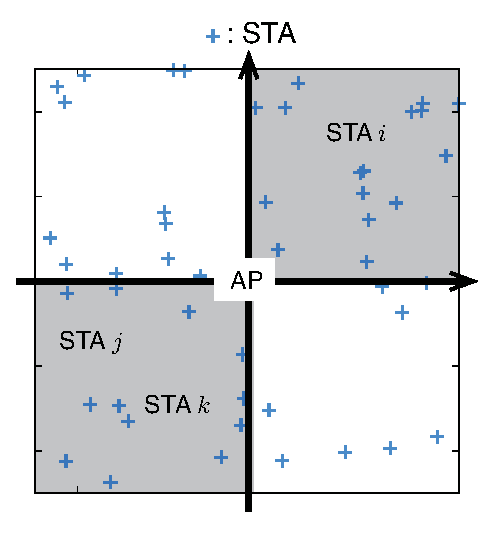
\epsfig{file=fig/time.eps, scale=0.6}
			\caption{位置によるSTAのグループ分け}
			\label{fig:time_image}
		\end{figure}
		本節では,最適化問題を解くための計算時間を削減する手法について検討する.
		第\ref{sec:opt}節で述べたように,APは最適化問題を定期的に解き確率$\pijk$を更新する.
		確率$\pijk$は,STAの参加離脱,移動による$\rijk$の変化,$d^{(j)}$,$d^{(k)}$の更新など状態の変化に追従するよう更新する必要があるため,
		数百ミリ秒単位で最適化問題を解く必要がある.
		提案方式の最適化問題は線形最適化問題であるが,Karmarkarの内点法~\cite{karmarkar}を用いる場合,
		計算量は変数の数$n$に対して$O(n^{3.5})$であり,指数的に増加する.
		変数の数は送受信STAの組み合わせの数$|{\mthc}|$であり,STA台数を$N$台,OFDMAの多重数を$M$とすると,
		最大で$(N+1)N^M-1$となる.
		そのため,$N$が大きくなると計算量が爆発的に大きくなる.
		\par
		そこで,本稿では計算時間削減の初期検討として,選択可能なSTA組を制限する手法を検討する.
		ある送受信STA組におけるスループットはユーザ間干渉が大きいほど減少する傾向にある.
		また,ユーザ間干渉の大きさはSTAの地理的位置に依存し,受信STAと送信STAとの距離が遠いほど干渉が小さくなる傾向にある.
		そこで,STAを位置によってグループ分けし特定のSTA組に限定することで組み合わせの数を削減する.
		\par
		STAの組み合わせをユーザ間干渉が小さくなる可能性が高い組み合わせのみに限定するため,
		下り通信を行うSTA $i$と上り通信を行う2台のSTA $j$,$k$がAPを中心として対角の位置に存在する組み合わせのみを最適化の対象とする.
		図\ref{fig:time_image}のようにAPを中心とした直交座標を設定し,それぞれのSTAがどの象限に位置するかによって4つのグループに分ける.
		そして,組み合わせの集合$\mthc$には,OFDMAとUFD通信を組み合わせる場合はSTA $i$と2台のSTA $j$,$k$は対角の象限,STA $j$と$k$は同じ象限に存在するような組み合わせ,UFD通信の場合はSTA$i$と$j$は対角の象限に存在する組み合わせのみを含める.

\section{シミュレーション評価}

	\begin{table}[t]
		\centering
		\caption{シミュレーション諸元}
		\label{tab:param}
		\begin{tabular}{cc} \hline
			領域の大きさ $L$ & 100\,m \\
			伝送速度 & シャノン容量 \\
			送信電力 & 15\,dBm \\
			雑音指数 & 10\,dB \\
			周波数帯 & 2.4\,GHz \\
			帯域幅(半二重,UFD通信) & 20\,MHz \\
			帯域幅(OFDMA)& 10Mhzずつ \\
			伝搬損失 & $30\log D + 40$\\
			&($D$: 送受信点間距離)\\
			自己干渉除去 & 110\,dB \\
			シミュレーション時間 & 10\,s \\\hline
		\end{tabular}
	\end{table}

	本章では提案手法の有効性をシミュレーションによって評価する.
	シミュレーションは最適化問題はMATLABにより計算し,そのほかの部分はC言語で作成したシミュレータによって行う.
	半二重通信のみを用いる場合,半二重通信とUFD通信を併用する従来方式~\cite{promac_fair}と,
	半二重通信,UFD通信,上りOFDMA,UFD通信と上りOFDMAの組み合わせの4方式を用いる提案方式を比較する.
	OFDMAによる多重化は簡単のため二多重までとし,チャネル幅は二等分するものとする.
	図\ref{fig:model}のように,1台のAPが $L=$100\,m四方の領域の中心に設置され,その周りに$N=50$台のSTAがランダムに配置されているとする.
	式\eqref{eq:etad}における$\eta_{\rm d}^{(i)}$には各STA共通の$1/[(N+1)N]$を,
	式\eqref{eq:etau}における$\eta_{\rm u}^{(l)}$には各STA共通の$1/(N+1)$を設定している.
	伝送速度はIEEE 802.11aに従う.
	上下通信ともに飽和トラヒックであり,APには1500\,Bの,STAには64\,Bのデータフレームが発生しているものとする.
	これは,トラヒックの多くがTCP-ACKを中心とする64\,B以下のフレームと1500\,Bのフレームによって占められるからである~\cite{traffic}.

		\begin{figure}[t]
			\centering
			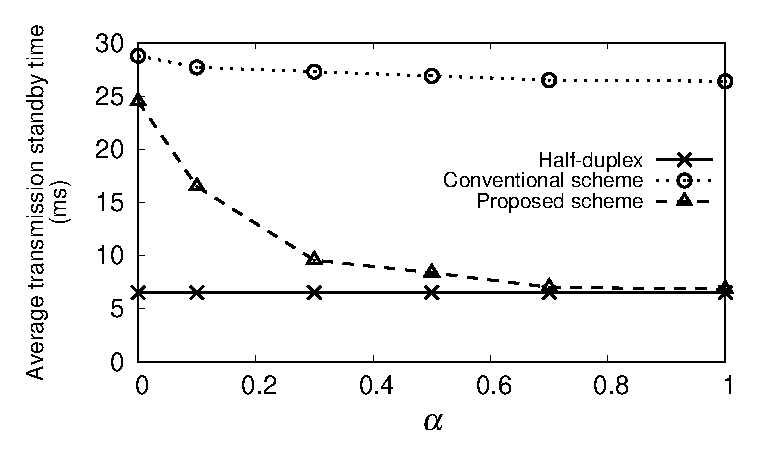
\epsfig{file=graph/delay.eps, scale=0.6}
			\caption{上り通信の平均遅延時間}
			\label{fig:delay}
		\end{figure}
		\begin{figure}[t]
			\centering
			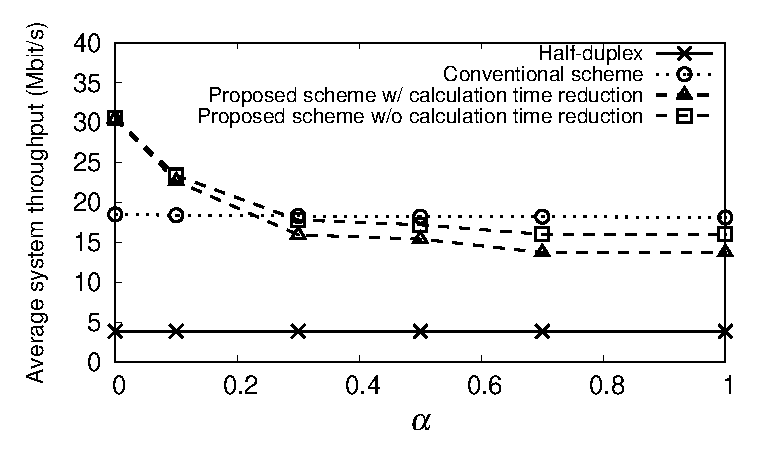
\epsfig{file=graph/thr.eps, scale=0.6}
			\caption{システムスループット}
			\label{fig:thr}
		\end{figure}
		\begin{figure}[t]
			\centering
			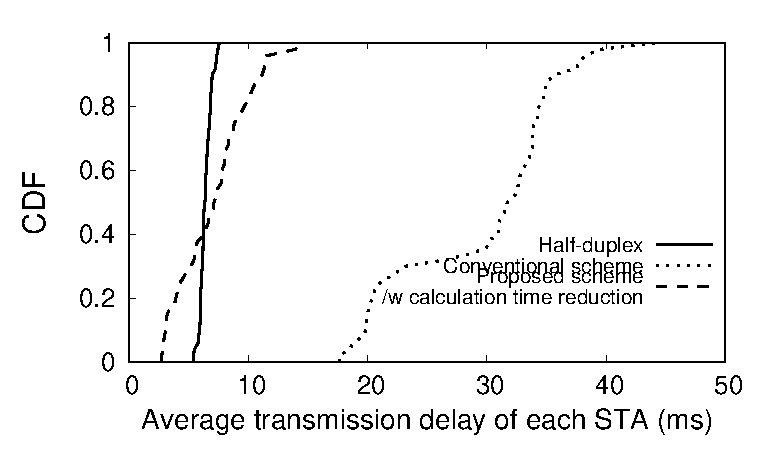
\epsfig{file=graph/cdf.eps, scale=0.6}
			\caption{ある試行における各STAの平均遅延時間のCDF}
			\label{fig:cdf}
		\end{figure}

		\par
		図\ref{fig:delay},\ref{fig:thr}にSTAの平均遅延時間とシステムスループットを示す.
		半二重通信とUFD通信を用いる従来方式の遅延時間は半二重通信と比べ20\,ms以上大きい.
		一方,提案方式はパラメータ$\alpha$を大きくすることで遅延時間を半二重通信と同等の値まで削減できている.
		しかし,$\alpha$が大きくなるにつれて,システムスループットが低下している.
		これは,最適化問題の目的関数において$d^{(j)},\ d^{(k)}$の項の影響が大きくなり,スループットの低下による利得の減少より遅延時間削減による利得向上が上回るためである.
		提案方式はシステムスループットは低下したものの,半二重通信に対しては3倍程度の値を維持しつつ,
		遅延時間を半二重通信と同等まで削減することができた.
		\par
		STA間の公平性を示すため,図\ref{fig:cdf}に各STA毎の平均遅延時間のCDF(Cumulative distribution functioin)を示す.
		半二重通信では全STAが平等に送信機会を獲得するため,STA間の遅延時間のばらつきは非常に小さい.
		提案方式は半二重通信には及ばないものの,従来方式と比べて大幅にばらつきが小さくなっており,
		遅延時間に対する公平性が高いことを示している,

		\begin{table}[t]
			\centering
			\caption{最適化問題を1回解くために必要な平均時間}
			\label{tab:time}
			\begin{tabular}{cc}
			 計算時間削減なし & 計算時間削減あり\\ \hline
			 803\,ms & 226\,ms \\\hline
			\end{tabular}
		\end{table}
%		\begin{figure}[t]
%			\centering
%			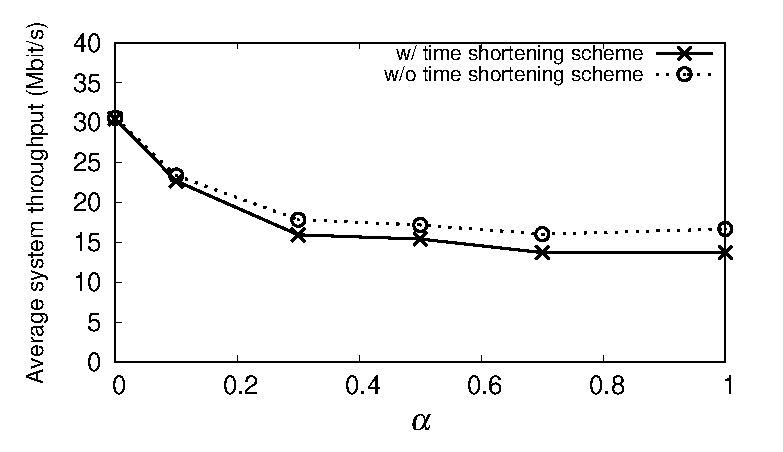
\epsfig{file=graph/thr_time.eps, scale=0.6}
%			\caption{システムスループットへの計算時間削減手法の影響}
%			\label{fig:thr_time}
%		\end{figure}

	\par
	次に計算時間について評価する.
	表\ref{tab:time}に第\ref{sec:time}節で述べた計算時間削減手法を用いた場合と用いない場合について,
	$\alpha=1$における最適化問題を一回解くために必要な平均時間を示す.
	計算時間を72\%削減できている一方,送受信STAの組み合わせを制限するため,利得の高い組み合わせまで除外されることがありシステムスループットが低下する.
	図\ref{fig:thr}より計算量削減手法を用いた場合でもシステムスループットの低下は最大18\%となった.
	簡易な方式ながら,システムスループットを大幅に低下させることなく,計算時間を削減することができた.
%	$\alpha$が小さいときには送信待機時間$d^{(j)},\ d^{(k)}$の影響が小さく,
%	干渉の小さな組み合わせが選ばれやすい.
%	干渉の小さな組み合わせは,APに対してSTA $i$とSTA $j$,$k$が対角の位置に存在している場合であり,
%	このような組み合わせは計算時間削減手法を用いていても除外されていないため,影響が少ないと考えられる.
%	一方,$\alpha$が大きいときには送信待機時間$d^{(j)},\ d^{(k)}$の影響が大きく,
%	例えある程度干渉が大きい組み合わせでも送信待機時間が大きいSTAを選ばざる負えない.
%	このような場合は,計算時間削減手法によって除外された組み合わせの中によりよい組み合わせが含まれてしまっていることがあるため,
%	システムスループットが低下してしまうと考えられる.

\section{まとめ}
	本稿では,UFD通信に上りOFDMAを適用するための送受信STA選択手法を提案した.
	STAの遅延時間が増大するというUFD通信の問題点を,上り通信をOFDMAにより多重化し,
	STAの送信機会を増加させることで改善を行った.
	更に,STAのグループ分けを行い最適化問題の変数の数を減らすことで,計算時間を削減する手法についても検討した.

\bibliographystyle{sieicej}
\bibliography{main2}

\end{document}
